\documentclass[conference]{IEEEtran}
\IEEEoverridecommandlockouts
% The preceding line is only needed to identify funding in the first footnote. If that is unneeded, please comment it out.
\usepackage{hyperref}
\usepackage{cite}
\usepackage{amsmath,amssymb,amsfonts}
\usepackage{algorithmic}
\usepackage{graphicx}
\usepackage{textcomp}
\usepackage{xcolor}
\def\BibTeX{{\rm B\kern-.05em{\sc i\kern-.025em b}\kern-.08em
    T\kern-.1667em\lower.7ex\hbox{E}\kern-.125emX}}
\begin{document}

\title{Analisis Profit dalam Model Biaya-Pendapatan Non-Linear}

\author{\IEEEauthorblockN{Muhammad Riyan Satrio Wibowo}
\IEEEauthorblockA{\textit{NPM: 2306229323} \\
\textit{Departemen Teknik Elektro}\\
\textit{Universitas Indonesia}\\
mriyansatriow@gmail.com}
}

\maketitle

\begin{abstract}
Laporan ini membahas analisis profit dalam model ekonomi di mana fungsi pendapatan dan biaya bersifat non-linear. Tujuan analisis ini adalah untuk menentukan kuantitas produksi yang menghasilkan profit maksimum serta menghitung total profit pada rentang produksi tertentu. Mengingat kompleksitas model, solusi analitik sulit diperoleh, sehingga digunakan pendekatan numerik. Metode Newton-Raphson diterapkan untuk menemukan titik profit maksimum dengan mencari akar dari turunan pertama fungsi profit. Turunan tersebut dihitung menggunakan centered finite difference. Selanjutnya, total profit dihitung melalui integrasi numerik menggunakan Simpson's Rule. Analisis dilakukan pada 5 dataset berbeda untuk membandingkan hasilnya.
\end{abstract}

\begin{IEEEkeywords}
metode numerik, optimisasi profit, newton-raphson, simpson's rule, model non-linear
\end{IEEEkeywords}

\section{Pendahuluan}
Dalam konteks produksi, perlu dilakukan analisis profit maksimum dan total profit untuk menentukan titik optimal produksi. Pendapatan diasumsikan meningkat secara linear pada awalnya, namun akan menurun secara non-linear setelah melewati titik tertentu karena adanya kejenuhan pasar. Di sisi lain, biaya akan semakin tinggi secara non-linear seiring peningkatan jumlah produksi. 

Karena bentuk fungsi yang kompleks dan non-linear, pendekatan numerik digunakan untuk melakukan analisis. Titik profit maksimum ditentukan menggunakan metode Newton-Raphson setelah menghitung turunan pertama profit secara numerik. Sementara itu, Simpson’s Rule digunakan untuk menghitung total profit dalam rentang produksi tertentu melalui pendekatan integrasi numerik. Metode ini memungkinkan analisis yang lebih akurat dalam kondisi di mana solusi analitik sulit diperoleh.

\section{Studi Literatur}
Analisis profit memerlukan model matematis untuk pendapatan dan biaya, serta metode numerik untuk optimisasi dan integrasi.

\subsection{Fungsi Pendapatan (Revenue)}
Fungsi pendapatan memodelkan pendapatan awal yang linear ($ax$) namun menurun secara non-linear (suku $-bx^3$) akibat kejenuhan pasar. Konsep ini merupakan dasar dalam teori organisasi industri.
\begin{equation}
R(x) = ax - bx^3
\label{eq:revenue}
\end{equation}
dengan:
\begin{itemize}
    \item $a$ : koefisien pendapatan linear
    \item $b$ : koefisien penurunan pendapatan
    \item $x$ : jumlah unit produksi
\end{itemize}

\subsection{Fungsi Biaya (Cost)}
Fungsi biaya mencakup biaya tetap ($e$) dan biaya variabel yang meningkat secara non-linear ($cx^2$ dan $de^{0.01x}$). Peningkatan ini menunjukkan adanya batasan produksi atau penurunan efisiensi saat produksi ditingkatkan.
\begin{equation}
C(x) = cx^2 + de^{0.01x} + e
\label{eq:cost}
\end{equation}
dengan:
\begin{itemize}
    \item $c$ : koefisien biaya kuadratik
    \item $d$ : koefisien biaya variabel
    \item $e$ : biaya tetap
\end{itemize}

\subsection{Fungsi Profit}
Fungsi profit, yang merupakan selisih antara pendapatan dan biaya. Fungsi inilah yang akan dioptimalkan untuk mencari kuantitas produksi paling menguntungkan.
\begin{equation}
P(x) = R(x) - C(x)
\end{equation}

\subsection{Optimisasi Profit dengan Metode Newton-Raphson}
Titik profit maksimum ditemukan saat turunan pertama profit bernilai nol ($P'(x)=0$). Metode Newton-Raphson digunakan untuk mencari akar dari fungsi turunan ini secara iteratif guna menemukan kuantitas produksi yang optimal.
\begin{equation}
x_{k+1} = x_k - \frac{P'(x_k)}{P''(x_k)}
\end{equation}

\subsection{Diferensiasi Numerik}
Karena kompleksitas fungsi, turunan pertama dan kedua profit tidak dihitung secara analitik, melainkan secara numerik. Metode \textit{centered finite difference} dipilih karena akurasinya yang terbilang baik.
\begin{equation}
P'(x) \approx \frac{P(x+h) - P(x-h)}{2h}
\end{equation}
\begin{equation}
P''(x) \approx \frac{P(x+h) - 2P(x) + P(x-h)}{h^2}
\end{equation}

\subsection{Total Profit dengan Simpson's 1/3 Rule}
Total profit pada rentang produksi dihitung melalui integrasi numerik. Simpson's 1/3 Rule diterapkan untuk mengaproksimasi nilai integral dari fungsi profit, memberikan estimasi total yang akurat.
\begin{multline}
\int_{a}^{b} f(x) dx \approx \frac{h}{3} \Big[ f(x_0) + 4\sum_{i=1,3,5}^{n-1} f(x_i) \\
+ 2\sum_{i=2,4,6}^{n-2} f(x_i) + f(x_n) \Big]
\end{multline}

\section{Data yang Digunakan}
Analisis ini menggunakan lima dataset untuk memodelkan berbagai skenario bisnis. Dataser yang digunakan disajikan pada Tabel \ref{tab:koefisien}.

\begin{table}[htbp]
\caption{Koefisien untuk 5 Set Data}
\begin{center}
\begin{tabular}{|c|c|c|c|c|c|}
\hline
\textbf{Dataset} & \textbf{$a$} & \textbf{$b$} & \textbf{$c$} & \textbf{$d$} & \textbf{$e$} \\
\hline
1 & 276.00 & 0.0010 & 0.18 & 105.00 & 3381.00 \\
\hline
2 & 235.00 & 0.0008 & 0.22 & 107.00 & 4004.00 \\
\hline
3 & 266.00 & 0.0005 & 0.21 & 151.00 & 3901.00 \\
\hline
4 & 286.00 & 0.0007 & 0.16 & 171.00 & 3037.00 \\
\hline
5 & 258.00 & 0.0006 & 0.14 & 197.00 & 3431.00 \\
\hline
\end{tabular}
\label{tab:koefisien}
\end{center}
\end{table}

Parameter-parameter tersebut dipilih untuk merepresentasikan berbagai skenario bisnis melalui variasi nilai koefisien:
\begin{itemize}
    \item \textbf{Pendapatan:} Nilai pendapatan linear ($a$) yang tinggi, berkisar antara 235 hingga 286, mensimulasikan harga jual awal yang tinggi. Hal tersebut diimbangi oleh koefisien penurunan ($b$) yang kecil (0.0005-0.0010), yang memodelkan efek kejenuhan pasar pada volume produksi yang sangat tinggi.
    \item \textbf{Biaya Operasional:} Koefisien biaya kuadratik ($c$) memiliki nilai yang relatif kecil (0.14-0.22), menggambarkan peningkatan biaya operasional yang bertahap seiring dengan meningkatnya skala produksi.
    \item \textbf{Biaya Variabel:} Terdapat variasi signifikan pada koefisien biaya eksponensial ($d$), dengan nilai dari 105 hingga 197. Nilai yang lebih tinggi, seperti pada Dataset 5 (197), mensimulasikan skenario di mana biaya melonjak drastis akibat kendala produksi pada volume tinggi.
    \item \textbf{Biaya Tetap:} Biaya tetap ($e$) berada di rentang nilai yang signifikan (3037-4004), merepresentasikan investasi awal atau biaya operasional dasar yang harus ditanggung terlepas dari jumlah produksi.
\end{itemize}

\section{Metode yang Digunakan}
Implementasi analisis profit menggunakan dua metode numerik utama untuk optimisasi dan integrasi, yang dieksekusi secara otomatis untuk setiap set data oleh program \texttt{profit.c}.

\subsection{Optimisasi Profit: Metode Newton-Raphson}
Metode Newton-Raphson digunakan untuk mencari kuantitas yang memberikan profit maksimum dengan menemukan akar dari turunan pertama fungsi profit ($P'(x)=0$). Metode ini dipilih karena:
\begin{itemize}
    \item Memiliki tingkat konvergensi kuadratik yang sangat cepat.
    \item Merupakan metode standar untuk masalah optimisasi berbasis gradien.
    \item Penggunaan turunan kedua ($P''(x)$) secara langsung dapat mengkonfirmasi bahwa titik yang ditemukan adalah titik maksimum.
\end{itemize}

\textbf{Algoritma Metode Newton-Raphson:}
\begin{algorithmic}
\STATE \textbf{Input:} $x_0$ (tebakan awal), toleransi $\epsilon$
\STATE \textbf{Output:} Kuantitas profit maksimum $x$
\REPEAT
    \STATE $P'(x_0) \leftarrow \text{hitung\_turunan\_pertama}(x_0)$
    \STATE $P''(x_0) \leftarrow \text{hitung\_turunan\_kedua}(x_0)$
    \IF{$|P''(x_0)| < \epsilon$}
        \RETURN error (turunan kedua terlalu kecil)
    \ENDIF
    \STATE $x_1 \leftarrow x_0 - P'(x_0) / P''(x_0)$
    \STATE $\text{selisih} \leftarrow |x_1 - x_0|$
    \STATE $x_0 \leftarrow x_1$
\UNTIL{$\text{selisih} < \epsilon$ atau mencapai iterasi maksimum}
\RETURN $x_0$
\end{algorithmic}

\subsection{Integrasi Profit: Simpson's 1/3 Rule}
Simpson's 1/3 Rule digunakan untuk menghitung total akumulasi profit pada rentang produksi tertentu ($\int P(x)dx$). Metode ini dipilih karena:
\begin{itemize}
    \item Memberikan akurasi yang lebih tinggi dibanding metode trapezoid dengan memodelkan kurva sebagai parabola.
    \item Sangat efisien untuk mengintegrasikan fungsi non-linear yang mulus.
\end{itemize}

\textbf{Algoritma Simpson's Rule:}
\begin{algorithmic}
\STATE \textbf{Input:} $x_{low}, x_{high}$ (batas integral), $n$ (jumlah interval)
\STATE \textbf{Output:} Total profit (nilai integral)
\STATE $h \leftarrow (x_{high} - x_{low}) / n$
\STATE $S \leftarrow P(x_{low}) + P(x_{high})$
\FOR{$i = 1$ to $n-1$}
    \STATE $x \leftarrow x_{low} + i \cdot h$
    \IF{$i \pmod 2 = 0$}
        \STATE $S \leftarrow S + 2 \cdot P(x)$
    \ELSE
        \STATE $S \leftarrow S + 4 \cdot P(x)$
    \ENDIF
\ENDFOR
\RETURN $(h / 3) \cdot S$
\end{algorithmic}

\section{Analisa Hasil}

\subsection{Analisis Komparatif Dataset}
Dari kelima dataset yang diuji, program berhasil menghitung kuantitas optimal untuk memaksimalkan profit. Berikut adalah rangkuman hasil komprehensif dari semua skenario:
\begin{itemize}
    \item \textbf{Rentang Kuantitas Optimal:} 227.67 – 283.93 unit
    \item \textbf{Rentang Profit Maksimum:} \$27,611.62 – \$46,324.28
    \item \textbf{Rentang Total Profit (0-500 unit):} \$4.12 juta – \$14.10 juta
\end{itemize}

Observasi penting dari hasil analisis:
\begin{itemize}
    \item Semua dataset menunjukkan titik profit maksimum yang konvergen pada rentang kuantitas yang relatif sempit, membuktikan robustnya model.
    \item \textbf{Dataset 4} menghasilkan profit tertinggi (\$46,324.28) berkat kombinasi pendapatan linear (\textit{a}) tertinggi dan biaya tetap (\textit{e}) terendah.
    \item \textbf{Dataset 2} mencatatkan profit terendah (\$27,611.62), yang disebabkan oleh pendapatan linear (\textit{a}) paling rendah dan biaya tetap (\textit{e}) tertinggi di antara semua skenario.
    \item Koefisien biaya variabel eksponensial (\textit{d}) terbukti menjadi faktor krusial yang membedakan total profit jangka panjang antar dataset.
\end{itemize}

Analisis komparatif secara visual disajikan pada Gambar \ref{fig:profits}. Grafik ini memplot fungsi profit untuk kelima dataset secara bersamaan, memungkinkan perbandingan langsung terhadap performa masing-masing model bisnis. Titik pada setiap kurva menandai profit maksimum yang dihitung, yang secara visual mengkonfirmasi bahwa skenario pada Dataset 4 adalah yang paling menguntungkan.

\vspace{1cm}
\begin{figure}[htbp]
\centering
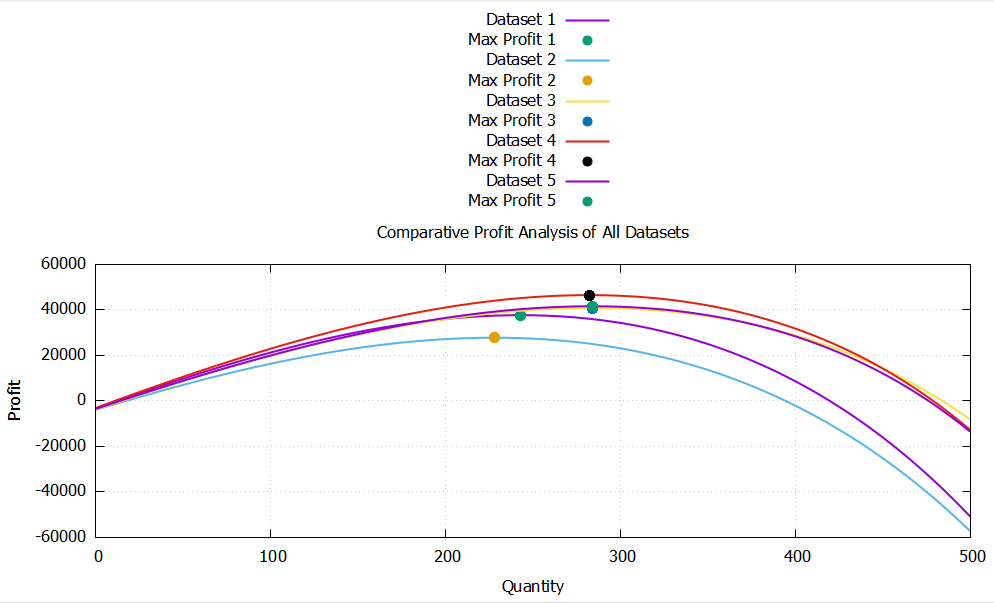
\includegraphics[width=\columnwidth]{plot_all_profits.png}
\caption{Perbandingan fungsi profit (P(x)) untuk kelima dataset. Titik pada setiap kurva menandai profit maksimum yang dihitung.}
\label{fig:profits}
\end{figure}
\vspace{1cm}

Selanjutnya, Gambar \ref{fig:derivatives} menyajikan perbandingan turunan pertama (P'(x)) dari fungsi profit untuk setiap dataset. Grafik ini menunjukkan laju perubahan profit. Titik di mana setiap kurva memotong garis horizontal y=0 adalah titik dimana kuantitas menghasilkan profit maksimum pada Gambar \ref{fig:profits}.

\begin{figure}[htbp]
\centering
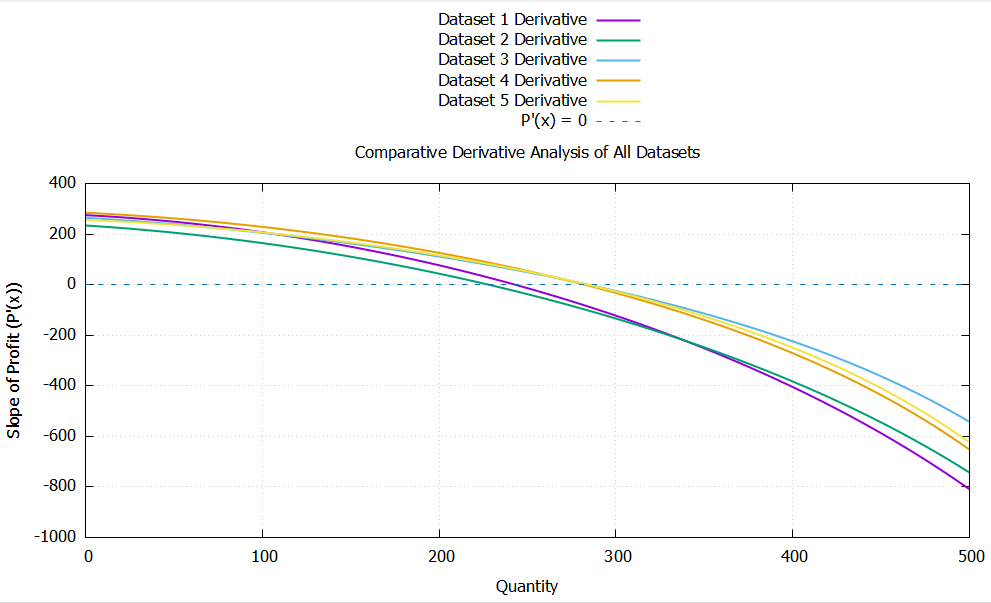
\includegraphics[width=\columnwidth]{plot_all_derivatives.png}
\caption{Perbandingan turunan pertama (P'(x)) dari fungsi profit. Titik potong dengan sumbu x menunjukkan lokasi profit maksimum.}
\label{fig:derivatives}
\end{figure}

\vspace{1cm}
\subsection{Detail Hasil per Dataset}

\subsubsection{Dataset 1}
\begin{itemize}
    \item \textbf{Model Matematis:}
    \begin{itemize}
        \item Revenue: \( R(x) = 276x - 0.001x^3 \)
        \item Cost: \( C(x) = 0.18x^2 + 105e^{0.01x} + 3381 \)
        \item Profit: \( P(x) = -0.001x^3 - 0.18x^2 + 276x - 105e^{0.01x} - 3381 \)
    \end{itemize}
    \item \textbf{Hasil Analisis:}
    \begin{itemize}
        \item Kuantitas Optimal : 242.71 unit
        \item Profit Maksimum  : \$37,516.67
        \item Total Profit (0-500) : \$8,136,661.78
    \end{itemize}
\end{itemize}

\subsubsection{Dataset 2}
\begin{itemize}
    \item \textbf{Model Matematis:}
    \begin{itemize}
        \item Revenue: \( R(x) = 235x - 0.0008x^3 \)
        \item Cost: \( C(x) = 0.22x^2 + 107e^{0.01x} + 4004 \)
        \item Profit: \( P(x) = -0.0008x^3 - 0.22x^2 + 235x - 107e^{0.01x} - 4004 \)
    \end{itemize}
    \item \textbf{Hasil Analisis:}
    \begin{itemize}
        \item Kuantitas Optimal : 227.67 unit
        \item Profit Maksimum  : \$27,611.62
        \item Total Profit (0-500) : \$4,129,012.48
    \end{itemize}
\end{itemize}

\subsubsection{Dataset 3}
\begin{itemize}
    \item \textbf{Model Matematis:}
    \begin{itemize}
        \item Revenue: \( R(x) = 266x - 0.0005x^3 \)
        \item Cost: \( C(x) = 0.21x^2 + 151e^{0.01x} + 3901 \)
        \item Profit: \( P(x) = -0.0005x^3 - 0.21x^2 + 266x - 151e^{0.01x} - 3901 \)
    \end{itemize}
    \item \textbf{Hasil Analisis:}
    \begin{itemize}
        \item Kuantitas Optimal : 283.93 unit
        \item Profit Maksimum  : \$40,667.61
        \item Total Profit (0-500) : \$12,511,061.22
    \end{itemize}
\end{itemize}

\subsubsection{Dataset 4}
\begin{itemize}
    \item \textbf{Model Matematis:}
    \begin{itemize}
        \item Revenue: \( R(x) = 286x - 0.0007x^3 \)
        \item Cost: \( C(x) = 0.16x^2 + 171e^{0.01x} + 3037 \)
        \item Profit: \( P(x) = -0.0007x^3 - 0.16x^2 + 286x - 171e^{0.01x} - 3037 \)
    \end{itemize}
    \item \textbf{Hasil Analisis:}
    \begin{itemize}
        \item Kuantitas Optimal : 282.04 unit
        \item Profit Maksimum  : \$46,324.28
        \item Total Profit (0-500) : \$14,106,568.23
    \end{itemize}
\end{itemize}

\subsubsection{Dataset 5}
\begin{itemize}
    \item \textbf{Model Matematis:}
    \begin{itemize}
        \item Revenue: \( R(x) = 258x - 0.0006x^3 \)
        \item Cost: \( C(x) = 0.14x^2 + 197e^{0.01x} + 3431 \)
        \item Profit: \( P(x) = -0.0006x^3 - 0.14x^2 + 258x - 197e^{0.01x} - 3431 \)
    \end{itemize}
    \item \textbf{Hasil Analisis:}
    \begin{itemize}
        \item Kuantitas Optimal : 283.74 unit
        \item Profit Maksimum  : \$41,433.63
        \item Total Profit (0-500) : \$12,422,127.33
    \end{itemize}
\end{itemize}

\section{Kesimpulan}
Implementasi analisis profit untuk model non-linear menggunakan metode Newton-Raphson dan Simpson's Rule berhasil:
\begin{itemize}
    \item Menentukan kuantitas produksi optimal yang memaksimalkan profit dengan akurasi tinggi untuk setiap skenario bisnis.
    \item Menghitung total akumulasi profit pada rentang produksi yang luas, memberikan gambaran potensi jangka panjang.
    \item Memberikan visualisasi komparatif yang jelas tentang profitabilitas dari berbagai model biaya-pendapatan.
    \item Mendemonstrasikan dampak signifikan dari setiap parameter, terutama biaya variabel dan pendapatan linear, terhadap profit maksimum.
\end{itemize}
Kombinasi metode numerik ini terbukti sebagai alat analisis yang kuat untuk pengambilan keputusan strategis dalam skenario bisnis non-linear yang kompleks, terutama dalam menentukan skala operasi yang paling menguntungkan.

\section{Link Github}
Source code lengkap dapat diakses melalui repositori GitHub berikut:
\url{https://github.com/r-ediewitsch/ProyekUAS_Komnum}

\section{Link Youtube}
Video penjelasan mengenai proyek ini dapat ditemukan di link berikut:
https://youtube.com/watch?v=video-id

\begin{thebibliography}{00}
\bibitem{b1} J. Tirole, \textit{The Theory of Industrial Organization}. Cambridge, MA: MIT Press, 1988.
\bibitem{b2} L. Cabral and M. Riordan, ``Dynamic Price Competition with Production Constraints,'' \textit{Journal of Economic Theory}, vol. 63, pp. 42--62, 1994.
\bibitem{b1} S. C. Chapra and R. P. Canale, \textit{Numerical Methods for Engineers}, 7th ed. New York: McGraw-Hill Education, 2015.
\bibitem{b_judd} K. L. Judd, \textit{Numerical Methods in Economics}. Cambridge, MA: The MIT Press, 1998.
\end{thebibliography}

\end{document}